\chapterimage{Dewatering.jpg} % Chapter heading image

\chapter{Part I - Practice Math Problems Solutions}

\section{Unit Conversions}\index{Unit Conversions}
\begin{enumerate}
\item Given 1 ft = 30.48 cm and 5,280 ft = mile, convert 3 miles to cm\\
Solution:\\
$3 \enspace \cancel{miles} * \dfrac{5,280 \enspace \cancel{ft}}{\cancel{mile}}*\dfrac{30.48 \enspace cm}{\cancel{ft}}=\boxed{482,803 \enspace cm}$

\item The wastewater flow to a treatment plant has a velocity of 61 cm/s. What is this velocity expressed in ft/min. Given: 1 ft = 30.48 cm\\
Solution:\\
$61 \enspace \dfrac{\cancel{cm}}{\cancel{s}} * \dfrac{ft}{30.48 \enspace \cancel{cm}}* \dfrac{60 \enspace \cancel{s}}{min} =  \boxed{120 \enspace ft/min}$\\

\item As an operator of a wastewater plant you are treating a flow of 21 MGD, what is the flow in gallons per minute?\\
Solution:\\
$\dfrac{21 \cancel{MG}}{\cancel{day}}*\dfrac{1,000,000 \enspace gal}{\cancel{MG}}*\dfrac{\cancel{day}}{24*60 \enspace min}=\boxed{\dfrac{14,583 \enspace gal}{min}}$\\
\end{enumerate}

\newpage

\section{Area \& Volume}\index{Area \& Volume}
\begin{enumerate}

\item A cylindrical tank is 10 feet in diameter and 20 feet in height. 'What is the approximate capacity in liters?\\
Solution:\\

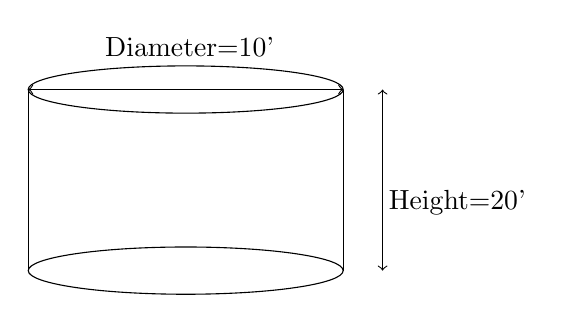
\begin{tikzpicture}
\draw (0,0) ellipse (2cm and 0.3cm);
\draw (0,-2.3) ellipse (2cm and 0.3cm);
\draw [-] (2,-2.3) -- (2,0);
\draw [<->] (-2,0) -- (2,0) node [midway, above=3mm] {\hspace{0.1cm}Diameter=10'}; 
\draw [<->] (2.5,-2.3) -- (2.5,0) node [midway, below] {\hspace{1.9cm}Height=20'};
%\draw [-] (0,-4) -- (2,-2.3);
%\draw [-] (0,-4) -- (-2,-2.3);
%\draw [-] (0,-4) -- (2,-2.3);
\draw [-] (-2,0) -- (-2,-2.3);
\end{tikzpicture}\\

$Volume=\dfrac{\pi}{4}D^2*H=0.785*10^2*20\cancel{ft^3}*7.48\dfrac{\cancel{gallons}}{\cancel{ft^3}}*3.78\dfrac{liters}{\cancel{gallons}}=\boxed{44,462 \enspace liters}$

\item What is the volume of water in a sedimentation basin 80 feet long, 28 feet wide and a 9.5 feet water depth? Give your answer in gallons.\\
Solution:\\
$Volume=80*28*9.5 \cancel{ft^3}*7.48\dfrac{gallons}{\cancel{ft^3}}=\boxed{159,174 \enspace gallons} $

\item How many gallons will 1,200 feet of 6-inch pipe hold?\\
Solution:\\
\begin{center}
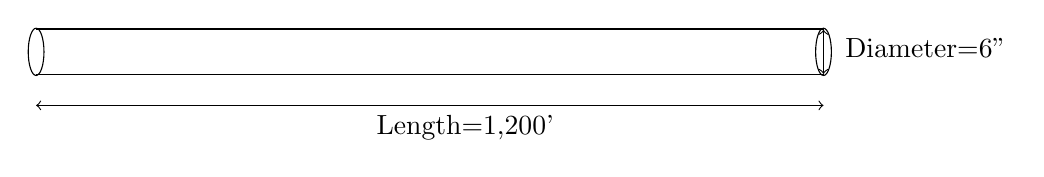
\begin{tikzpicture}
\draw (0,0) ellipse (0.1cm and 0.3cm);
\draw (10,0) ellipse (0.1cm and 0.3cm);
\draw [-] (0,-0.29) -- (10,-0.29);
\draw [-] (0,0.29) -- (10,0.29);
\draw [<->] (10,-0.28) -- (10,0.28) node [midway, below=-3mm] {\hspace{2.6cm}Diameter=6"};
\draw [<->] (0,-.68) -- (10,-.68)node [midway, below] {\hspace{0.9cm}Length=1,200'};
\end{tikzpicture}
\end{center}
$Volume=\dfrac{\pi}{4}D^2*L=0.785*\Big(\dfrac{6}{12}\Big)^2*1200\cancel{ft^3}*7.48\dfrac{gallons}{\cancel{ft^3}}=\boxed{1,762 \enspace gallons}$

\item What is the surface area of a cylinder 80 ft diameter and 25 ft height?  Cylindrical part surface area only. Disregard the floor and roof areas.\\
Solution:\\
\begin{center}
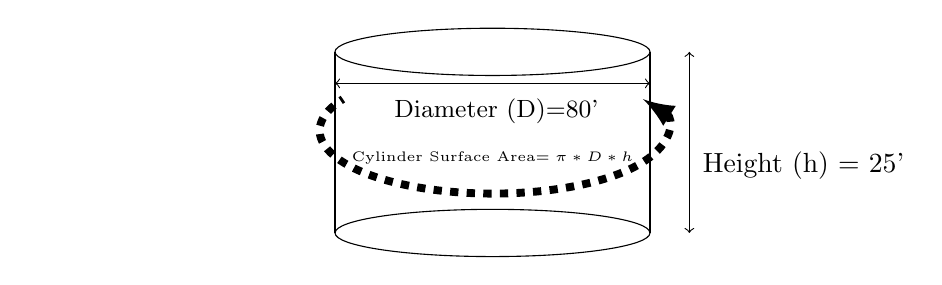
\begin{tikzpicture}[mydashed/.style={dashed,dash phase=2pt}]
\draw (0,0) ellipse (2cm and 0.3cm) node [midway, above=-2.4mm] {};
\draw (0,-2.3) ellipse (2cm and 0.3cm) node [midway, below=2.05cm] {};
\draw [-] (2,-2.3) -- (2,0);
%\draw [<->] (-2,0) -- (2,0); 
\draw [<->] (2.5,-2.3) -- (2.5,0) node [midway, below] {\hspace{2.9cm}Height (h) = 25'};
\draw [<->] (-2,-0.4) -- (2,-0.4) node [midway, below=0.7mm] {\hspace{0.1cm}\small{Diameter (D)}=80'};
%\draw [-] (0,-4) -- (2,-2.3);
%\draw [-] (0,-4) -- (-2,-2.3);
%\draw [-] (0,-4) -- (2,-2.3);
\draw [-] (-2,0) -- (-2,-2.3) node [midway, below] {\hspace{4cm}\tiny{Cylinder Surface Area$=\pi*D*h$}};
\draw [-latex, mydashed, line width=1mm, rotate=-90] (0.6,-1.9) arc [start angle=-120, end angle=120, x radius=0.8cm, y radius=2.2cm];
%\draw [-latex, thick, rotate=-95] (0,0) arc [start angle=-190, end angle=160, x radius=1cm, y radius=2cm];
\end{tikzpicture}\\
\end{center}
$Surface \enspace area \enspace of \enspace cylinder=\pi*D*h=3.14*80*25=\boxed{6,280ft^2}$

\item If the surface area of a clarifier is 5,025$ft^2$, what is its circumference?\\
Solution:\\
$Surface \enspace area=\dfrac{\pi}{4}*D^2 \enspace \implies 5025ft^2=0.785*D^2 ft^2\implies D^2=\dfrac{5025}{0.785} \implies D=\sqrt{6401.3}=80ft \implies \enspace Circumference=\pi*D=3.14*80ft=\boxed{251ft}$

\item How many gallons of paint will be required to paint the inside walls of a 40 ft long x 65 ft wide x 20 ft high tank if the paint coverage is 150 sq. ft per gallon.  Note:  We are painting walls only.  Disregard the floor and roof areas.\\
Solution:\\
\begin{center}
\begin{tikzpicture}
	%%% Edit the following coordinate to change the shape of your
	%%% cuboid
      
	%% Vanishing points for perspective handling
	\coordinate (P1) at (-7cm,1.5cm); % left vanishing point (To pick)
	\coordinate (P2) at (8cm,1.5cm); % right vanishing point (To pick)

	%% (A1) and (A2) defines the 2 central points of the cuboid
	\coordinate (A1) at (0em,0cm); % central top point (To pick)
	\coordinate (A2) at (0em,-2cm); % central bottom point (To pick)

	%% (A3) to (A8) are computed given a unique parameter (or 2) .8
	% You can vary .8 from 0 to 1 to change perspective on left side
	\coordinate (A3) at ($(P1)!.8!(A2)$); % To pick for perspective 
	\coordinate (A4) at ($(P1)!.8!(A1)$);

	% You can vary .8 from 0 to 1 to change perspective on right side
	\coordinate (A7) at ($(P2)!.7!(A2)$);
	\coordinate (A8) at ($(P2)!.7!(A1)$);

	%% Automatically compute the last 2 points with intersections
	\coordinate (A5) at
	  (intersection cs: first line={(A8) -- (P1)},
			    second line={(A4) -- (P2)});
	\coordinate (A6) at
	  (intersection cs: first line={(A7) -- (P1)}, 
			    second line={(A3) -- (P2)});

	%%% Depending of what you want to display, you can comment/edit
	%%% the following lines

	%% Possibly draw back faces

	\fill[gray!40] (A2) -- (A3) -- (A6) -- (A7) -- cycle; % face 6
	\node at (barycentric cs:A2=1,A3=1,A6=1,A7=1) {};
	
	\fill[gray!50] (A3) -- (A4) -- (A5) -- (A6) -- cycle; % face 3
	\node at (barycentric cs:A3=1,A4=1,A5=1,A6=1) {\tiny Wall - W*H};
	
	\fill[gray!10, opacity=0.2] (A5) -- (A6) -- (A7) -- (A8) -- cycle; % face 4
	\node at (barycentric cs:A5=1,A6=1,A7=1,A8=1) {\tiny Wall - L*H};
	
	\fill[gray!10,opacity=0.5] (A1) -- (A2) -- (A3) -- (A4) -- cycle; % f2
	\node at (barycentric cs:A1=1,A2=1,A3=1,A4=1) {\tiny Wall - L*H};
	
	\fill[gray!40,opacity=0.2] (A1) -- (A4) -- (A5) -- (A8) -- cycle; % f5
	\node at (barycentric cs:A1=1,A4=1,A5=1,A8=1) {};	
	
	\draw[thick,dashed] (A5) -- (A6);
	\draw[thick,dashed] (A3) -- (A6);
	\draw[thick,dashed] (A7) -- (A6);

	%% Possibly draw front faces

	%\fill[orange] (A1) -- (A8) -- (A7) -- (A2) -- cycle; % face 1
	\node at (barycentric cs:A1=1,A8=1,A7=1,A2=1) {\tiny Wall - W*H};
	


	%% Possibly draw front lines
	\draw[thick] (A1) -- (A2);

	\draw[<->] (-1.8,0.38) -- (-1.8,-1.3)node [midway, above=-1.8mm] {\hspace{-1.3cm}\tiny Height=20'};
	\draw[<->] (-1.6,-1.4) -- (-.3,-2.1)node [midway, above=-2.6mm] {\hspace{-1.3cm}\tiny Length=45'};
	\draw[<->] (2.6,-1.13) -- (0.2,-2.2)node [midway, below=.6mm] {\hspace{1.2cm}\tiny Width=65'};
	\draw[thick] (A3) -- (A4);
	\draw[thick] (A7) -- (A8);
	\draw[thick] (A1) -- (A4);
	\draw[thick] (A1) -- (A8);
	\draw[thick] (A2) -- (A3);
	\draw[thick] (A2) -- (A7);
	\draw[thick] (A4) -- (A5);
	\draw[thick] (A8) -- (A5);
	
	% Possibly draw points
	% (it can help you understand the cuboid structure)
%	\foreach \i in {1,2,...,8}
%	{
%	  \draw[fill=black] (A\i) circle (0.15em)
%	    node[above right] {\tiny \i};
%	}
	% \draw[fill=black] (P1) circle (0.1em) node[below] {\tiny p1};
	% \draw[fill=black] (P2) circle (0.1em) node[below] {\tiny p2};
\end{tikzpicture}\\
\end{center}
2 Walls W*H + 2 Walls L*H = $2*65*20ft^2 + 2*40*20ft^2= 2,600+1,600=4,200ft^2$\\
$\implies @150\dfrac{ft^2}{gal} \enspace paint \enspace coverage \enspace \rightarrow \enspace \dfrac{4,200\cancel{ft^2}}{150\dfrac{\cancel{ft^2}}{gal}}=\boxed{28 \enspace gallons}$

\item What is the circumference of a 100 ft diameter circular clarifier?\\
Solution:\\
$Circumference=\pi*D=3.14*100ft=\boxed{314ft}$

\item If the surface area of a clarifier is 5,025$ft^2$, what is its diameter?\\
Solution:\\
$Surface \enspace area=\dfrac{\pi}{4}*D^2 \enspace \implies 5025ft^2=0.785*D^2 ft^2\implies D^2=\dfrac{5025}{0.785} \implies D=\sqrt{6401.3}=\boxed{80ft}$

\end{enumerate}

\section{Concentration}\index{Concentration}
\begin{enumerate}
\item A 6.35\% solution is is equivalent to {\underline{\hspace{1cm}}} mg/l\\
Answer:\\
63,500 mg/l\\
\end{enumerate}
\section{Pounds Formula}\index{Pounds Formula}
\begin{enumerate}
\item An operator dissolves 1,200 lbs of a chemical in 12,000 gallons of water, what is the resultant concentration in mg/l, of the chemical solution?\\
Solution:\\
$Concentration \enspace \dfrac{mg}{l}=\dfrac{lbs}{Volume \enspace MG \enspace * \enspace 8.34}$\\
$Concentration \enspace \dfrac{mg}{l}=\dfrac{1,200}{0.012 \enspace * \enspace 8.34}=\boxed{\dfrac{11,990 \enspace mg}{l} \enspace or \enspace 1.2\% \enspace solution}$\\
\textbf{Note:}\\  
12,000 gallons was converted to MG by dividing by 1,000,000\\
$12,000 \enspace gallons * \dfrac{1 MG}{1,000,000 \enspace gallons}$\\
\end{enumerate}
\section{Removal Efficiency}\index{Removal Efficiency}
\begin{enumerate}

\item What is the \% removal efficiency if the influent concentration is 10 mg/L and the effluent concentration is 2.5 mg/L?\\
$Removal \enspace Rate (\%) = \dfrac{In-Out}{In}*100 \implies \dfrac{10-2.5}{10}*100=\boxed{75\%}$

\item If a plant removes 35\% of the influent BOD in the primary treatment and 85\% of the remaining BOD in the secondary system, what is the BOD of the raw wastewater if the BOD of the final effluent is 20mg/l \\
Solution:\\
\tikzstyle{block} = [rectangle, draw, fill=red!40, 
    text width=6em, text centered, rounded corners, minimum height=3em]
\tikzstyle{arrow} = [draw, -latex']
\begin{figure}[!h]
\centering
\begin{tikzpicture}[node distance =1.5cm, auto]
    \draw ++(0,0) node [block] (Primary) {Primary};
    
   \node[node distance=1.9in] (dummy_in) [left of=Primary] {Influent BOD};
   \node[node distance=1.9in] (dummy_out) [right of=Primary] {Primary BOD Out};
	\node (Removal) [below of=Primary, yshift=-0in] {$Removal \enspace Efficiency=35\% $};
    \path [arrow] (dummy_in)-- (Primary)  node [above] {\hspace{-4.8cm}$X \enspace mg/l \enspace$} node [below] {};
    \path [arrow] (Primary) -- (dummy_out)  node [above] {\hspace{-4.9cm}$0.65X \enspace mg/l$} node [below] {};
   \draw[arrow] (Process) -- (Removal);
\end{tikzpicture}
\end{figure}

\tikzstyle{block} = [rectangle, draw, fill=red!40, 
    text width=6em, text centered, rounded corners, minimum height=3em]
\tikzstyle{arrow} = [draw, -latex']
\begin{figure}[!h]
\centering
\begin{tikzpicture}[node distance =1.5cm, auto]
    \draw ++(0,0) node [block] (Secondary) {Secondary};
    
   \node[node distance=1.9in] (dummy_in) [left of=Secondary] {Primary BOD Out};
   \node[node distance=1.9in] (dummy_out) [right of=Secondary] {Secondary BOD Out};
	\node (Removal) [below of=Secondary, yshift=-0in] {$Removal \enspace Efficiency=85\% $};
    \path [arrow] (dummy_in)-- (Secondary)  node [above] {\hspace{-4.8cm}$0.65X \enspace mg/l \enspace$} node [below] {\hspace{-5cm}$100 \enspace mg/l$};
    \path [arrow] (Secondary) -- (dummy_out)  node [above] {\hspace{-4.9cm}$20 \enspace mg/l$} node [below] {\hspace{-4.9cm}$15 \enspace mg/l$};
   \draw[arrow] (Process) -- (Removal);
\end{tikzpicture}
\end{figure}
\vspace{0.3cm}
For the Secondary process:\\
$\dfrac{In}{Out}: \enspace \dfrac{0.65X}{20}=\dfrac{100}{15} \implies X \enspace mg/l=\dfrac{100*20}{15*0.65}=\boxed{205 \enspace mg/l}$\\

\vspace{0.3cm}
Alternate Solution \#1

$\xrightarrow[
				\text{X}\dfrac{mg}{l}
			]
			{
			\text{Influent BOD}
			}
 \boxed{Primary}
 \xrightarrow[
 				\text{X-0.35X=X*(1-0.35)=0.65X}\dfrac{mg}{l}
 			]
 			{
 			\text{Primary Effluent BOD}
 			}
 \boxed{Secondary}
 \xrightarrow[
				\text{0.65X-0.5525X=(0.65-0.5525)X=0.0975X }
			 ]
			{
			\text{Secondary Effluent BOD}
			}
$\\

\hspace{2.8cm}$\downarrow$ {\tiny(0.35X)BOD Removed}\hspace{3.2cm}$\downarrow$ {\tiny(0.65*0.85)X = 0.5525X BOD Removed}\\
$\implies 0.0975X=20 \implies X=\dfrac{20}{0.0975}=\boxed{205\dfrac{mg}{l}}$\\

\vspace{0.3cm}

Alternate Solution \#2:\\
$\xrightarrow[\text{X}\dfrac{mg}{l}]{\text{Influent BOD}}\boxed{Primary}\xrightarrow[\text{0.65X}]{\text{Primary Effluent BOD}}\boxed{Secondary}\xrightarrow[\text{(0.65*0.15)X}]{\text{Secondary Effluent BOD}}$\\
\hspace{2.8cm}$\downarrow$ {\tiny(0.35X)BOD Removed}\hspace{2.2cm}$\downarrow$ {\tiny(0.65X*0.85)BOD Removed}\\

Primary Effluent BOD = Influent BOD * (1-Primary BOD Removal), and\\
Secondary Effluent BOD=[Primary Effluent BOD]*(1-Secondary BOD Removal)\\
Secondary Eff. BOD=[Influent BOD * (1-Primary BOD Removal)]*(1-Secondary BOD Removal)\\

Therefore, 20 = [X*(1-0.35)] * (1-0.85)= X*0.65*0.15\\
$\implies 20 \enspace \dfrac{mg}{l}= 0.0975X \implies X=\dfrac{20}{0.0975}=\boxed{205 \enspace \dfrac{mg}{l}}$\\

\item Calculate the inlet concentration if the outlet concentration is 80 mg/l and the process removal efficiency is 60\%\\

\tikzstyle{block} = [rectangle, draw, fill=red!40, 
    text width=6em, text centered, rounded corners, minimum height=3em]
\tikzstyle{arrow} = [draw, -latex']
\begin{figure}[!h]
\centering
\begin{tikzpicture}[node distance =1.5cm, auto]
    \draw ++(0,0) node [block] (Process) {Process};
   \node[node distance=1.5in] (dummy_in) [left of=Process] {In};
   \node[node distance=1.5in] (dummy_out) [right of=Process] {Out};
	\node (Removal) [below of=Process, yshift=-0in] {$Removal \enspace Efficiency=60\%$};
    \path [arrow] (dummy_in)-- (Process)  node [above] {\hspace{-4.39cm}$Xmg/l$} node [below] {\hspace{-4.39cm}$100mg/l$};
    \path [arrow] (Process) -- (dummy_out)  node [above] {\hspace{-3.cm}80mg/l} node [below] {\hspace{-3cm}40mg/l};
   \draw[arrow] (Process) -- (Removal);
\end{tikzpicture}
\end{figure}

$\dfrac{In}{Out} \enspace : \enspace \dfrac{Actual \enspace inlet \enspace  (X)}{80}=\dfrac{100}{100-60}$\\
$\implies \dfrac{Actual \enspace inlet \enspace  (X)}{80}=2.5$\\    
Rearranging the equation:   $Actual \enspace inlet (X)=2.5*80 = \boxed{200 mg/l}$\\

\item Calculate the outlet concentration if the inlet concentration is 80 mg/l and the process removal efficiency is 60\%\\
Solution:\\

\tikzstyle{block} = [rectangle, draw, fill=red!40, 
    text width=6em, text centered, rounded corners, minimum height=3em]
\tikzstyle{arrow} = [draw, -latex']
\begin{figure}[!h]
\centering
\begin{tikzpicture}[node distance =1.5cm, auto]
    \draw ++(0,0) node [block] (Process) {Process};
   \node[node distance=1.5in] (dummy_in) [left of=Process] {In};
   \node[node distance=1.5in] (dummy_out) [right of=Process] {Out};
	\node (Removal) [below of=Process, yshift=-0in] {$Removal \enspace Efficiency=60\%$};
    \path [arrow] (dummy_in)-- (Process)  node [above] {\hspace{-4.39cm}$80mg/l$} node [below] {\hspace{-4.39cm}$100mg/l$};
    \path [arrow] (Process) -- (dummy_out)  node [above] {\hspace{-3.cm}$Xmg/l$} node [below] {\hspace{-3cm}40mg/l};
   \draw[arrow] (Process) -- (Removal);
\end{tikzpicture}
%\caption[MFCC]{Diagrama en bloques del cálculo de las MFCC para un frame.}
%\label{MFCC}
\end{figure}
\vspace{0cm}
$\dfrac{Out}{In} \enspace:\enspace\dfrac{Actual \enspace Outlet (X)}{80}=\dfrac{100-60}{100}$\\
$\implies \dfrac{Actual \enspace Outlet (X)}{80} =0.4$\\
$\implies Actual \enspace  Outlet (X) = 0.4 * 80 = \boxed{32 mg/l}$\\

\end{enumerate}

\section{Flow and Velocity}\index{Flow and Velocity}
\begin{enumerate}
\item A wastewater channel is 3.25 feet wide and is conveying a wastewater flow of 3.5 MGD. The wastewater flow is 8 inches deep. Calculate the velocity of this flow.\\
Solution:\\
\includegraphics[scale=0.5]{ChannelFlow3}\\
$Q=V*A \implies V=\dfrac{Q}{A}$\\
$\implies V\dfrac{ft}{s}=\dfrac{3.5\dfrac{\cancel{MG}}{\cancel{day}}*\dfrac{1000000\cancel{gal}}{\cancel{MG}}*\dfrac{ft^{\cancel{3}}}{7.48\cancel{gal}}*\dfrac{\cancel{day}}{(1440*60)s}}{(3.25*0.75)\cancel{ft^2}}=\boxed{2.2\dfrac{ft}{s}}$

\item A plastic float is dropped into a wastewater channel and is found to travel 10 feet in 4.2 seconds. The channel is 2.4 feet wide and is flowing 1.8 feet deep. Calculate the flow rate of this wastewater in cubic feet per second.\\
Solution:\\
$Q=V*A$\\
$\implies Q\Big(\dfrac{ft^3}{s}\Big)=\dfrac{10ft}{4.2s}*(2.4*1.8)ft^2=\boxed{10.3\dfrac{ft^3}{s}}$
\item A 12 inch pipe conveys sewage at 2.6 feet per second.  What is the flow expressed in MGD?
Solution:\\
\includegraphics[scale=0.5]{PipeFlow}\\
$Q=V*A$\\
$Q=2.6\dfrac{\cancel{ft}}{\cancel{s}}*0.785*1^2\cancel{ft^2}*7.48\dfrac{\cancel{gal}}{ft^3}*\dfrac{MG}{1,000,000\cancel{gal}}*\dfrac{(1440*60)\cancel{s}}{day}=\boxed{1.3MGD}$\\

\item A sewer line to a wastewater treatment plant is 12 miles long. If the wastewater is flowing at 2.2 fps, approximately.  How long will it take for wastewater to reach the plant?\\
Solution:\\
$time \enspace to \enspace reach \enspace plant \enspace (hrs)=\dfrac{\cancel{s}}{2.2\cancel{ft}}*\dfrac{5280\cancel{ft}}{\cancel{mile}}*12\cancel{miles}*\dfrac{hrs}{(60*60)\cancel{s}}=\boxed{8hrs}$  
\end{enumerate}
\section{Preliminary Treatment}\index{Preliminary Treatment}
\begin{enumerate}
\item On an average a 12.5 yd. load of grit is hauled to the landfill once every 20 days. Plant flow averages 12.5 MGD. Calculate the rate of grit collection in ft$^3$/MG.\\
Solution:\\
$Grit Removal\Big(\dfrac{ft^3}{MG}\Big)=\dfrac{12.5\cancel{yd^3}}{ 20\cancel{days}}*\dfrac{27ft^3}{ \cancel{yd^3}}*\dfrac{\cancel{day}}{12.5MG}=\boxed{1.4\dfrac{ft^3}{MG}}$

\item On an average, 2 inches of grit is collected and removed every day in a 2.2 feet wide, 205 feet long grit channel.  Knowing the average flow through that grit channel is 10 MGD calculate the rate of grit collection in ft$^3$/MG\\
Solution:\\
Grit volume accumulated:  $\dfrac{2}{12}ft*(2.2*205)ft^2=\dfrac{75.16ft^3}{day}$
Grit Collection: $\dfrac{\dfrac{75.16ft^3}{\cancel{day}}}{\dfrac{10MG}{\cancel{day}}}=\boxed{7.5\dfrac{ft^3}{MG}}$ 
\end{enumerate}

\section{Primary Treatment} \index{Primary Treatment}
\begin{enumerate}
\item A circular clarifier receives a flow of 11 MGD.  If the clarifier is 90 ft. in diameter and is 12 ft. deep, what is: a) the hydraulic/surface loading rate, b) weir overflow rate, and c) clarifier detention time in hours?\\
Solution:\\
a) Hydraulic/surface loading rate:\\
$Clarifier \enspace hydraulic \enspace loading \enspace 	\Big(\dfrac{gpd}{ft^2}\Big) ==\dfrac{\dfrac{11\cancel{MG}}{{day}}*\dfrac{10^6gal}{\cancel{MG}}}{0.785*90^2 ft^2}=\boxed{1,730gpd/ft^2}$\\
b) Weir overflow rate:\\ 
$Weir \enspace overflow \enspace rate \Big(\dfrac{gpd}{ft}\Big) =\dfrac{\dfrac{11\cancel{MG}}{{day}}*\dfrac{10^6gal}{\cancel{MG}}}{3.14*90 ft}=\boxed{38,924gpd/ft}$\\
c) Clarifier detention time:\\
$Clarifier \enspace detention \enspace time \enspace (hr) = 	\dfrac{ Clarifier \enspace volume (cu.ft \enspace or \enspace gal)}{Influent \enspace flow \enspace (cu.ft \enspace or \enspace gal)/hr)}$\\
$Clarifier \enspace detention \enspace time \enspace (hr) = 	\dfrac{(0.785*90^2*15)\cancel{ft^3}}{\dfrac{11\cancel{MG}}{\cancel{day}}*\dfrac{10^6\cancel{gal}}{\cancel{MG}}*\dfrac{\cancel{ft^3}}{7.48\cancel{gal}}*\dfrac{\cancel{day}}{24hrs}}=\boxed{2hrs}$\\

\item At a 2.5 MGD wastewater treatment plant the primary clarifier has a detention time of 2 hours. How many gallons does this clarifier hold?\\

Solution:\\
\vspace{0.2cm}
$Clarifier \enspace detention \enspace time \enspace (hr) = 	\dfrac{ Clarifier \enspace volume (gal)}{Influent \enspace flow \enspace (gal/hr)}$\\
\vspace{0.2cm}
$ \implies Clarifier \enspace volume (gal)=Clarifier \enspace detention \enspace time \enspace (hr)*Influent \enspace flow \enspace (gal/hr)$\\
\vspace{0.2cm}
$ \implies Clarifier \enspace volume (gal)= \Big(2 \enspace hrs\Big)*\Big(2.5*10^6 \enspace \dfrac{gal}{day}*\dfrac{day}{24 \enspace hrs}\Big)=\boxed{208,333 \enspace gals}$\\

\end{enumerate}
\section{Pumping}\index{Pumping}
\begin{enumerate}
\item A sludge pump is set to pump 5 minutes each hour. It pumps at the rate of 35 gpm. How many gallons of sludge are pumped each day?\\
Solution:\\
$\dfrac{35 \enspace gal \enspace sludge}{\cancel{min}}*\dfrac{5 \enspace \cancel{min}}{\cancel{hr}} *\dfrac{24 \enspace \cancel{hr}}{day}=\boxed{\dfrac{4,200 \enspace gallons}{day}}$\\

\item A community has a total flow of 15 MGD which is passed through a primary treatment plant which removes 60\% of the TSS and 35\% of the BOD. The average strength of the influent is 400 mg/l TSS and 275 mg/l BOD. If the total solids of the raw sludge is 5\%, how many cu. ft of sludge is pumped daily?\\
Solution:\\
$lbs \enspace solids \enspace removed=(400*0.60)mg/l*15MGD*8.34=30,024lbs \enspace solids \enspace per \enspace day$
$$\dfrac{ft^3\enspace sludge}{day}= \dfrac{30,924 \enspace \cancel{lbs \enspace solids}}{day} * \dfrac{1 \enspace \cancel{lb \enspace sludge}}{0.05\enspace \cancel{lbs \enspace solids}}*\dfrac{\cancel{gal \enspace sludge}}{8.34\cancel{lb \enspace sludge}}*\dfrac{ft^3 \enspace sludge}{7.48 \enspace \cancel{gal}}=\boxed{9,626\dfrac{ft^3 \enspace sludge}{day}} $$

\item How many lbs of solids are removed daily by a primary clarifier treating a 6 MGD flow if the average influent TSS concentration is 300 mg/l and the clarifier TSS removal efficiency is 67\%?\\
Solution:\\
As the removal efficiency is 67\%, 0.67 * 300 mg/l = 201 mg/l solids are removed.\\
The total lbs removed can be calculated using the lbs formula.\\
$ \dfrac{lbs \enspace solids}{day}= 6 MGD* 201  \dfrac{mg \enspace  SS}{l}*8.34=\boxed{10,058 \dfrac{lbs \enspace solids}{day}}$
\end{enumerate}
